\documentclass[lettersize,journal,onecolumn,12pt]{IEEEtran}
\hyphenation{op-tical net-works semi-conduc-tor}
\usepackage{times}
\usepackage{epsfig}
\usepackage{graphicx}
\usepackage{amsmath}
\usepackage{amssymb}
\usepackage{multirow}
\usepackage{booktabs}
\usepackage[table]{xcolor}
\usepackage{listings}
\usepackage{footnote}
\usepackage{bm}
\usepackage{cite}
\usepackage[normalem]{ulem}
\useunder{\uline}{\ul}{}
\usepackage{amsfonts}
\usepackage[numbers,sort]{natbib}
\usepackage[dvipsnames]{xcolor}
\usepackage{setspace}
\usepackage{xcolor}
\onehalfspacing
\usepackage[bottom=2.0cm, top=2.0cm,left=2cm,right=2cm]{geometry}

%%%%%%%%%%%%%%%%%%%%%%%%%%%%%%%%%%%%%%%%%%%%%%%%%%%%%%%%%%%%%%%%%%%%%%%%
%% ★★★★★★★★★★★★★★★★★  待填清单（给作者本人看）  ★★★★★★★★★★★★★★★★★
%%
%% PDF 里所有黄底红字的 [[TO FILL Fx: ...]] 都是需要你填的空。
%% 现在只剩 4 处 F1–F4，都在频率可视化图 Fig.6（abl1019）上，全文搜 "FILLIN" 即可定位：
%%
%%   F1: Fig.6（FAM高低频可视化图 abl1019）中那张样本图来自哪个数据集
%%       的测试集（例如 Crack500）。共出现两处（正文句子里一处、图注一处），
%%       两处填同一个数据集名。
%%   F2: 该样本上 FAM (Full 全频融合) 配置的单图 IoU 数值（图(c)）。
%%   F3: 该样本上 FAM (High-Freq 仅高频) 配置的单图 IoU 数值（图(d)）。
%%   F4: 该样本上 FAM (Low-Freq 仅低频) 配置的单图 IoU 数值（图(e)）。
%%       ↑ F2–F4：用保存的三个消融模型对这张图各跑一次，算单图 IoU 即可。
%%
%% 【失败案例图 Fig.7 已改用 FANet 自己的真实预测裁片 failure_cases.pdf，
%%   不再需要你出图或填数据集/IoU（原 F5/F6/F7 已取消）。】
%%
%% 填完后把 \FILLIN{...} 整个命令删掉换成真实数字/名称即可；
%% 只要 PDF 里不再有黄块，就说明没有漏填。
%% ★★★★★★★★★★★★★★★★★★★★★★★★★★★★★★★★★★★★★★★★★★★★★★★★★★★★★★★★★★
%%%%%%%%%%%%%%%%%%%%%%%%%%%%%%%%%%%%%%%%%%%%%%%%%%%%%%%%%%%%%%%%%%%%%%%%

% 醒目的橙色占位标记 + 黄色高亮底色：投稿前必须全部替换掉，PDF 里不再有黄底即为填完
\definecolor{fillorange}{RGB}{200,60,0}
\definecolor{fillyellow}{RGB}{255,242,0}
\newcommand{\FILLIN}[1]{\colorbox{fillyellow}{\textcolor{fillorange}{\textbf{[[TO FILL #1]]}}}}

\begin{document}

\definecolor{myblue}{RGB}{0,0,255}

\title{Response to Review of paper (Second-Round / Minor Revision):\\
Harnessing Frequency-Aware Network for Crack Detection in Road-Perceptive Autonomous Vehicles Scene}

\author{Senyun Kuang, Yintao Wei,

Yang Liu, and Xiaobo Qu,~\IEEEmembership{Senior Member,~IEEE}
}

\markboth{Submit to IEEE Transactions on Cybernetics}%
{Shell \MakeLowercase{\textit{et al.}}: Bare Demo of IEEEtran.cls for IEEE Journals}

\maketitle

\textbf{Dear Associate Editor and Reviewers:}

We sincerely thank you for the constructive feedback on our revised manuscript
``Harnessing Frequency-Aware Network for Crack Detection in Road-Perceptive Autonomous Vehicles Scene''
(CYB-E-2025-10-3956).
We are encouraged that Reviewer~2 is fully satisfied with the previous revision and recommends acceptance,
and we are grateful to the Associate Editor and Reviewer~1 for the remaining suggestions,
all of which concern the clarity and completeness of the presentation.

In this second-round revision, we have carefully addressed every remaining comment. Specifically, we have
(i) clarified the representativeness and selection criteria of all qualitative visualizations and added
per-sample quantitative metrics to the corresponding captions;
(ii) restructured the descriptions of the proposed modules (FAM, T-M, and HFM) in Sections~III-B and III-C
into an ``intuition-first'' style, providing a concise high-level explanation of each module before the mathematical
formulation and consolidating the previously scattered equation-by-equation commentary;
(iii) added a new subsection ``Failure Cases and Limitations'' (Section~IV-H) that presents representative failure
examples and analyzes the boundary conditions of the proposed method; and
(iv) updated the Related Work section with recent (2024--2026) publications from journals and conferences,
including papers from IEEE Transactions on Cybernetics.

For clarity of marking: all text that is newly added or modified \emph{in this round} is highlighted in
\textcolor{red}{red} in the revised manuscript, while the red markings of the previous round have been restored
to black.

Below, we address each comment from the Associate Editor and the reviewers in turn.
The comments are labelled in bold and blue, followed by our responses.

\clearpage

\tableofcontents
\newpage

%%%%%%%%%%%%%%%%%%%%%%%%%%%%%%%%%%%%%%%%%%%%%%%%%%%%%%%%%%%%%%%%%%%%%%%%
\section{Response to Associate Editor}
%%%%%%%%%%%%%%%%%%%%%%%%%%%%%%%%%%%%%%%%%%%%%%%%%%%%%%%%%%%%%%%%%%%%%%%%

{\color{BlueGreen} \textbf{Comments to the Author:}

\textbf{The revised manuscript has been substantially improved; however, further clarification is still needed
regarding the representativeness of the visualizations, presentation of the proposed modules, and discussion of
failure cases and limitations. I therefore recommend revision before acceptance.
To put your contributions into the context of the most recent research, please update your Related Work section
to include relevant references that have appeared in the past two years in conferences and journals, including
from this Transaction.}}

\textbf{Response:}
We sincerely appreciate your positive assessment of the previous revision and your time in handling our manuscript.
All the remaining concerns have been fully addressed in this round:

\begin{itemize}
    \item \textbf{Representativeness of the visualizations.}
    We now explicitly state the selection criteria of every qualitative figure, label the exact configuration used in
    each frequency-based visualization, and report the per-sample quantitative metric (IoU) of each visualized example
    directly in the caption, so that the qualitative and quantitative evidence are connected.
    Please see our detailed response to \textbf{Reviewer~1, Comment~1}.

    \item \textbf{Presentation of the proposed modules.}
    Sections~III-B and III-C have been restructured in an ``intuition-first'' style: each module (FAM, T-M, and HFM)
    now begins with a concise, high-level explanation of its purpose and design rationale before any mathematical
    expression, and the previously scattered equation-by-equation commentary has been consolidated and condensed.
    Please see our detailed response to \textbf{Reviewer~1, Comment~2}.

    \item \textbf{Failure cases and limitations.}
    A new subsection, \textbf{``Failure Cases and Limitations'' (Section~IV-H)}, has been added. It presents
    representative failure examples grouped into three dominant failure modes, analyzes why FANet struggles in these
    conditions, and discusses the practical boundary conditions and future directions.
    Please see our detailed response to \textbf{Reviewer~1, Comment~3}.

    \item \textbf{Related Work update.}
    We have updated the Related Work section with recent publications that appeared in the past two years in
    journals and conferences, including works from IEEE Transactions on Cybernetics.
    The newly added text and references are listed below.
\end{itemize}

\textcolor{red}{In the revised manuscript, the following paragraph has been added to Section~II (Related Work):}

%%%%%%%%%%%%%%%%%%%%%%%%%%%%%%%%%%%%%%%%%%%%%%%%%%%%%%%%%%%%%%%%%%%%%%%%
%% 新增文献段：7 篇均已联网核实（TCYB×2 + TITS/CVPR/ESWA 裂缝检测×3 + 频域×2）
%%%%%%%%%%%%%%%%%%%%%%%%%%%%%%%%%%%%%%%%%%%%%%%%%%%%%%%%%%%%%%%%%%%%%%%%
\textcolor{red}{
More recent studies from the past two years further advance both crack detection and frequency-aware
representation learning. On the crack-detection side, UP-CrackNet~\cite{TITS24_UPCrackNet} formulates road crack
detection as unsupervised adversarial image restoration to remove the dependence on pixel-wise annotations;
SCSegamba~\cite{CVPR25_SCSegamba} designs a lightweight structure-aware vision Mamba that captures crack morphology
and texture with minimal computational cost; and an ultra-lightweight Mamba network with frequency-domain feature
extraction has been developed for pavement tiny-crack segmentation~\cite{ESWA25_MambaFreqCrack}.
On the frequency-modeling side, FreqFusion~\cite{TPAMI24_FreqFusion} rectifies feature fusion for dense prediction
with adaptive low-/high-pass filters, and FSEL~\cite{ECCV24_FSEL} entangles frequency and spatial representations
for camouflaged object detection. Closely related inspection and segmentation problems have also been actively
studied in IEEE Transactions on Cybernetics, including zero-shot industrial anomaly detection with hybrid
vision--language prompts~\cite{TCYB25_AnomalyVLM} and contrastive transformer-based segmentation of subtle
structures~\cite{TCYB24_CTNet}. These advances confirm the growing interest in spectral cues and efficient
architectures; however, they either address generic dense prediction or treat frequency information as an auxiliary
enhancement, leaving a deeply coupled frequency--spatial representation dedicated to road crack detection --- the
focus of FANet --- largely unexplored.
}

The above paragraph has been added to the end of \textbf{Section~II (Related Work)}, and the seven newly cited
works are: two from IEEE Transactions on Cybernetics
(AnomalyVLM, TCYB 2025~\cite{TCYB25_AnomalyVLM}; CTNet, TCYB 2024~\cite{TCYB24_CTNet}),
three recent crack-detection studies
(UP-CrackNet, T-ITS 2024~\cite{TITS24_UPCrackNet}; SCSegamba, CVPR 2025~\cite{CVPR25_SCSegamba};
ultra-lightweight Mamba--frequency network, ESWA 2025~\cite{ESWA25_MambaFreqCrack}),
and two recent frequency-aware representation studies
(FreqFusion, TPAMI 2024~\cite{TPAMI24_FreqFusion}; FSEL, ECCV 2024~\cite{ECCV24_FSEL}).\\[10pt]

\clearpage

%%%%%%%%%%%%%%%%%%%%%%%%%%%%%%%%%%%%%%%%%%%%%%%%%%%%%%%%%%%%%%%%%%%%%%%%
\section{Response to Reviewer 1}
%%%%%%%%%%%%%%%%%%%%%%%%%%%%%%%%%%%%%%%%%%%%%%%%%%%%%%%%%%%%%%%%%%%%%%%%

{\color{BlueGreen} \textbf{General Comments:}

\textbf{In this paper, the authors propose FANet, a frequency–spatial synergistic framework for crack detection that
integrates a Frequency-Aware Module (FAM), a Tri-Merge decoder (T-M), and a Hybrid Fusion Module (HFM). The revised
manuscript provides expanded technical explanations, ablation studies involving low-/high-/full-frequency variants of
FAM, and frequency-based visual comparisons. The work addresses a meaningful problem in pavement crack analysis and
shows clear improvements over baseline models. However, several issues still require clarification or refinement
before the paper can be accepted.}}

\textbf{Response:}
We sincerely thank the reviewer for the careful reading of our revised manuscript, the accurate summary of our
contributions, and the constructive suggestions. All three remaining comments have been fully addressed in this
round, as detailed below.\\[10pt]

%%%%%%%%%%%%%%%%%%  R1-Q1  %%%%%%%%%%%%%%%%%%%%%%%%
{\color{BlueGreen} \textbf{Q1 Comments to the Author:}

\textbf{The manuscript includes frequency-based visualizations (high/low/fusion), but the representativeness and
selection criteria of these examples should be clarified. The authors should explicitly state whether the provided
samples are typical, randomly selected, or chosen as illustrative cases, and each visualization should clearly label
the specific configuration used. Adding the corresponding quantitative metric of each visualized sample to the
caption would help readers connect qualitative and quantitative evidence more directly.}}

\textbf{Response:}
We thank the reviewer for this valuable suggestion. In the revised manuscript, we have made three changes to clarify
the representativeness of the frequency-based visualizations:

\begin{enumerate}
    \item \textbf{Selection criteria stated explicitly.}
    We now explicitly state in Section~IV-G that the sample shown in the frequency-based visualization (Fig.~6) is a
    \emph{typical case chosen as an illustrative example} (not randomly sampled, and not a best-performing case):
    it simultaneously contains a wide trunk crack and hairline branches on coarsely textured pavement, which is the
    condition under which the differences among the three FAM configurations are most visible.
    A corresponding statement of the selection criteria has also been added for the qualitative comparison figure
    (Fig.~5) in Section~IV-F.

    \item \textbf{Configuration of each panel labelled.}
    The caption of Fig.~6 now explicitly maps each panel to the exact configuration used in the ablation study
    (Table~II): panel~(c) is produced by \emph{FAM (Full)}, panel~(d) by \emph{FAM (High-Freq only)}, and panel~(e)
    by \emph{FAM (Low-Freq only)}.

    \item \textbf{Per-sample metrics added to the caption.}
    The per-sample IoU of each visualized prediction is now reported in the caption of Fig.~6, directly connecting
    the qualitative visualization with the quantitative evidence in Table~II.
\end{enumerate}

\textcolor{red}{In the revised manuscript, the following text has been added to Section~IV-G (Ablation Studies):}

%%%%%%%%%%%%%%%%%%%%%%%%%%%%%%%%%%%%%%%%%%%%%%%%%%%%%%%%%%%%%%%%%%%%%%%%
%% 【待填 F1】下面这段红字里的 \FILLIN{F1: ...} 要换成该样本所属数据集名，
%%            例如 Crack500。注意：图注里还有一处 F1，两处保持一致。
%%%%%%%%%%%%%%%%%%%%%%%%%%%%%%%%%%%%%%%%%%%%%%%%%%%%%%%%%%%%%%%%%%%%%%%%
\textcolor{red}{
To clarify the representativeness of the frequency-based visualization, the sample in Fig.~6
is a typical case selected from the \FILLIN{F1: dataset name, e.g. Crack500} test set as an illustrative example,
rather than a randomly drawn or best-performing image: it simultaneously contains a wide trunk crack and hairline
branches on coarsely textured pavement, the condition under which the differences among the three FAM configurations
in Table~II are most visible. Panels (c)--(e) are produced by the \emph{FAM (Full)}, \emph{FAM (High-Freq)}, and
\emph{FAM (Low-Freq)} configurations of Table~II, respectively, and the per-sample IoU of each panel is reported in
the caption to connect the qualitative and quantitative evidence.
}

\textcolor{red}{The caption of Fig.~6 has been rewritten as follows (the figure is reproduced below; figure/table numbers in the quoted text refer to the revised manuscript):}

\begin{figure}[!hbpt]
\centering
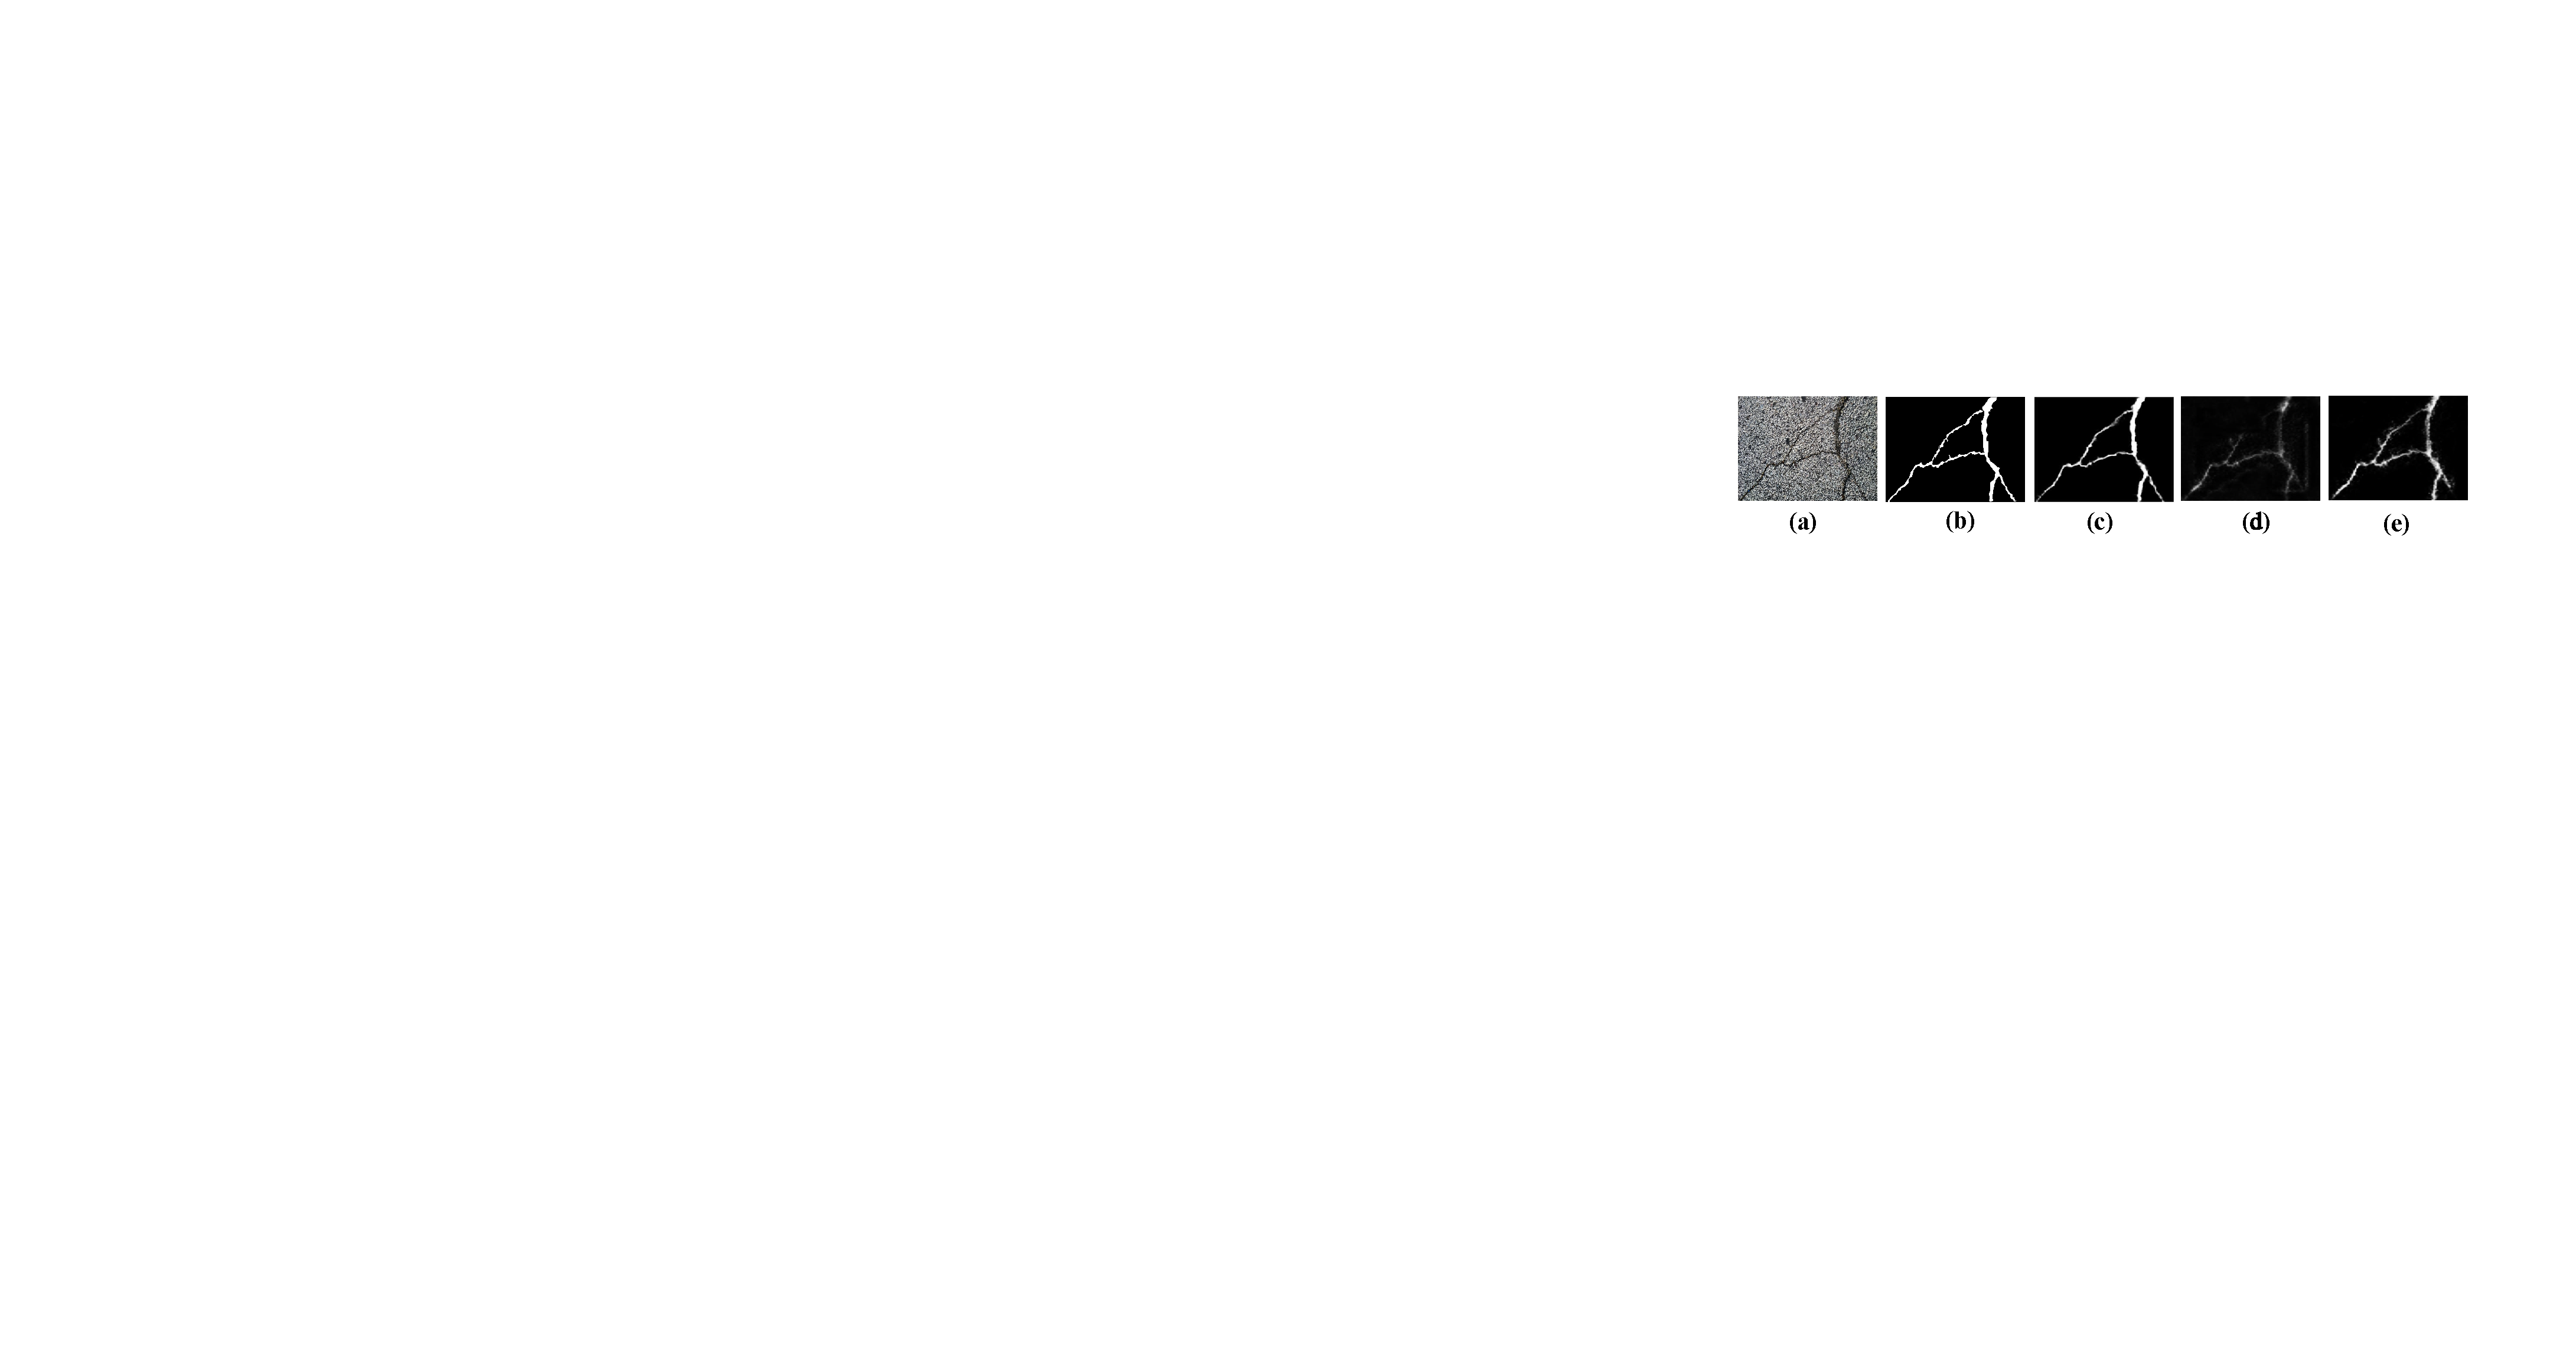
\includegraphics[width=0.85\linewidth]{Fig/abl1019.pdf}
%%%%%%%%%%%%%%%%%%%%%%%%%%%%%%%%%%%%%%%%%%%%%%%%%%%%%%%%%%%%%%%%%%%%%%%%
%% 【待填 F1/F2/F3/F4】图注中的四个橙色空：
%%   F1 = 样本所属数据集名（与上一段一致）
%%   F2 = 图(c) FAM (Full)      在这张样本上的单图 IoU，如 0.71
%%   F3 = 图(d) FAM (High-Freq) 在这张样本上的单图 IoU
%%   F4 = 图(e) FAM (Low-Freq)  在这张样本上的单图 IoU
%% 计算方法：用消融实验保存的三个模型分别对这张图推理，
%%           对预测二值化后与 GT 算 IoU（与论文 AIU 同一二值化阈值即可）。
%%%%%%%%%%%%%%%%%%%%%%%%%%%%%%%%%%%%%%%%%%%%%%%%%%%%%%%%%%%%%%%%%%%%%%%%
\caption{\textcolor{red}{Qualitative comparison of the three FAM configurations in Table~II on a typical sample
selected from the \FILLIN{F1: dataset name} test set as an illustrative case.
(a) Input. (b) Ground truth.
(c) Prediction of \emph{FAM (Full)}, which fuses the high- and low-frequency branches, per-sample IoU $=$
\FILLIN{F2: IoU of (c)}.
(d) Prediction of \emph{FAM (High-Freq only)}, per-sample IoU $=$ \FILLIN{F3: IoU of (d)}.
(e) Prediction of \emph{FAM (Low-Freq only)}, per-sample IoU $=$ \FILLIN{F4: IoU of (e)}.
The full-fusion configuration preserves both the main crack contour and the hairline branches, which is consistent
with the quantitative gains reported in Table~II.}}
\label{ablavis_rebuttal}
\end{figure}

\textcolor{red}{In addition, the following sentence has been added to Section~IV-F (Qualitative Results) to state the
selection criteria of the method-comparison figure (Fig.~5):}

\textcolor{red}{
The examples in Fig.~5 are typical cases selected from the test sets of the five datasets to cover the dominant
challenge conditions --- thin hairline cracks, coarse pavement texture, shadows and uneven illumination, and
crack-like distractors --- rather than randomly sampled or best-performing images; all methods are compared on
identical inputs.
}\\[10pt]

%%%%%%%%%%%%%%%%%%  end R1-Q1  %%%%%%%%%%%%%%%%%%%%%%%%


%%%%%%%%%%%%%%%%%%  R1-Q2  %%%%%%%%%%%%%%%%%%%%%%%%
{\color{BlueGreen} \textbf{Q2 Comments to the Author:}

\textbf{The overall descriptions of FAM, T-M, and HFM---particularly in Sections III-B and III-C---remain verbose and
would benefit from a clearer separation between intuition and formalism. Providing a concise, high-level explanation
of each module's purpose before introducing the mathematical expressions would significantly improve readability and
help interdisciplinary readers better understand the design motivations.}}

\textbf{Response:}
We thank the reviewer for this insightful suggestion, which has significantly improved the readability of the method
section. In the revised manuscript, Sections~III-B and III-C have been restructured following exactly the principle
suggested by the reviewer --- a clear separation between intuition and formalism:

\begin{enumerate}
    \item \textbf{Intuition first.} Each of the three modules (FAM, T-M, and HFM) now begins with a concise
    ``\emph{Design intuition}'' paragraph that explains, in plain language and without any equation, what problem the
    module solves and why it is designed this way.

    \item \textbf{Formalism afterwards, condensed.} The mathematical formulation follows the intuition paragraph.
    The previously scattered equation-by-equation commentary (several separate explanatory passages inserted after
    Eqs.~(1)--(4) in the last revision) has been consolidated into brief remarks, and overlapping explanations of the
    FAM mechanism, which appeared three times in slightly different wording, have been merged into a single passage.
    As a result, Sections~III-B and III-C are now \emph{shorter} than in the previous version while conveying the
    same technical content.
\end{enumerate}

\textcolor{red}{In the revised manuscript, the newly added ``Design intuition'' paragraphs are shown below:}

\textcolor{red}{
\textbf{(Section~III-B, before the formulation of FAM)}
\textbf{Design intuition of FAM.} Road cracks appear as sparse and sharp intensity discontinuities embedded in slowly
varying pavement context. In the feature space, the former concentrates in the high-frequency band, whereas the
latter dominates the low-frequency band. The FAM is therefore designed to (i) decompose each backbone feature into a
high-frequency and a low-frequency component, (ii) let the two components exchange complementary information, so that
edge responses acquire contextual support and contour responses are cleansed of texture noise, and (iii) adaptively
re-weight and merge the two bands with learnable gates. The output is a frequency-balanced feature in which crack
evidence is amplified relative to the background texture. The remainder of this subsection formalizes these three
steps.
}

\textcolor{red}{
\textbf{(Section~III-B, before the formulation of the T-M decoder)}
\textbf{Design intuition of T-M.} The T-M decoder aggregates the frequency-aware features of the three deepest
levels: deeper features indicate \emph{where} a crack is likely to exist, while shallower ones describe its shape
more precisely. Multiplying adjacent levels retains only the responses that are confirmed by both, yielding a clean
coarse localization map $S_1$.
}

\textcolor{red}{
\textbf{(Section~III-C, before the formulation of HFM)}
\textbf{Design intuition of HFM.} The HFM addresses two questions during refinement: \emph{where to refine} --- the
coarse map $S_g$ acts as a spatial prior that amplifies crack-relevant regions of the deeper feature; and \emph{what
to keep} --- a channel-level association between adjacent layers determines which high-resolution details are
consistent with this prior and should be preserved. Both operations are lightweight, so the refinement improves
accuracy at a marginal computational cost. The following formulation details the two steps.
}

In addition, the redundant explanatory passages of the previous round have been merged and condensed (the removed
redundancies are not marked in red, to keep the marking readable). We believe the method section is now
significantly easier to follow, especially for interdisciplinary readers.\\[10pt]

%%%%%%%%%%%%%%%%%%  end R1-Q2  %%%%%%%%%%%%%%%%%%%%%%%%


%%%%%%%%%%%%%%%%%%  R1-Q3  %%%%%%%%%%%%%%%%%%%%%%%%
{\color{BlueGreen} \textbf{Q3 Comments to the Author:}

\textbf{The paper would benefit from a short subsection discussing typical failure cases or limitations. Presenting a
small number of representative failure examples and briefly analyzing why FANet struggles in those conditions would
provide a more balanced understanding of the model's behavior and practical boundary conditions.}}

\textbf{Response:}
We thank the reviewer for this constructive suggestion, which makes the experimental analysis more balanced.
In the revised manuscript, we have added a new subsection, \textbf{``Failure Cases and Limitations''
(Section~IV-H)}, placed after the ablation studies. It presents representative failure examples --- taken directly
from FANet's own predictions on the hardest crack categories --- grouped into two dominant failure modes, analyzes
the underlying reasons within the frequency-aware design, and summarizes the practical boundary conditions and future
directions of FANet.

\textcolor{red}{In the revised manuscript, the newly added subsection is shown below (figure numbers in the quoted text refer to the revised manuscript, where the failure-case figure is Fig.~7; it is reproduced below):}

\textcolor{red}{
\textbf{IV-H. Failure Cases and Limitations.}
Although FANet achieves state-of-the-art performance on all five datasets, it still struggles under two identifiable
conditions. Fig.~7 shows representative failure cases drawn from FANet's own predictions on the most challenging crack
categories; in each column the top is the input image and the bottom is the predicted crack map.
}

\textcolor{red}{
\textbf{(1) Low-contrast and camouflaged cracks $\rightarrow$ fragmentation.} When a crack blends into the pavement
and its intensity contrast is low, the high-frequency response of FAM becomes weak and intermittent, while the
low-frequency contour prior is too smooth to bridge the gaps. Consequently, a single continuous crack is broken into
disconnected blobs or short segments, as in Fig.~7(a) and~(b).
}

\textcolor{red}{
\textbf{(2) Fine hairline cracks $\rightarrow$ under-segmentation.} When cracks are only a few pixels wide, the
frequency evidence they produce is faint relative to the surrounding pavement texture. Thin branches are then weakly
activated or missed and the predicted mask becomes broken and low in confidence, as in Fig.~7(c).
}

\textcolor{red}{
These two modes delineate the practical boundary condition of the proposed design: FANet implicitly assumes that
cracks constitute the dominant sparse high-frequency anomaly of the scene, an assumption that is violated when the
contrast is very low or the crack is extremely thin. In addition, two limitations are worth noting. First, the
two-step coarse-to-fine pipeline introduces extra inference cost compared with single-pass lightweight detectors, as
reflected by the FPS comparison in Table~I. Second, FANet is trained with the binary cross-entropy loss only and
imposes no explicit topological continuity constraint, which partially explains the fragmented predictions above. We
plan to explore topology-aware objectives, contrast-adaptive frequency gating, and complementary sensing modalities
(e.g., depth or infrared imaging) to push these boundaries in future work.
}

\begin{figure}[!hbpt]
\centering
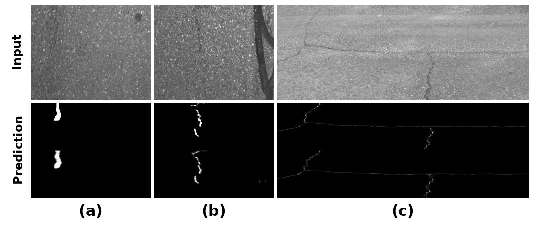
\includegraphics[width=0.95\linewidth]{Fig/failure_cases.pdf}
\caption{\textcolor{red}{Representative failure cases of FANet, taken from its own predictions on the hardest crack
categories. In each column the top is the input image and the bottom is the predicted crack map. (a) A camouflaged
crack is fragmented into two disconnected blobs; (b) a low-contrast crack is broken into short segments; (c) fine
hairline cracks are weakly activated and partly missed.}}
\label{failure_rebuttal}
\end{figure}

\vspace{6pt}

%%%%%%%%%%%%%%%%%%  end R1-Q3  %%%%%%%%%%%%%%%%%%%%%%%%

\clearpage

%%%%%%%%%%%%%%%%%%%%%%%%%%%%%%%%%%%%%%%%%%%%%%%%%%%%%%%%%%%%%%%%%%%%%%%%
\section{Response to Reviewer 2}
%%%%%%%%%%%%%%%%%%%%%%%%%%%%%%%%%%%%%%%%%%%%%%%%%%%%%%%%%%%%%%%%%%%%%%%%

{\color{BlueGreen} \textbf{Comments to the Author:}

\textbf{The authors have addressed all my concerns. I recommend acceptance. Thanks.}}

\textbf{Response:}
We sincerely thank the reviewer for the positive evaluation of our revised manuscript and for recommending
acceptance. The reviewer's constructive comments in the previous round have contributed greatly to improving the
quality of this work.\\[10pt]

\clearpage

{\small
\bibliographystyle{IEEEtran}
\bibliography{IEEEfull}
}

\end{document}
